%----------------------------------------------------------------------------------------
%	PACKAGES AND OTHER DOCUMENT CONFIGURATIONS
%----------------------------------------------------------------------------------------

\documentclass[11pt]{article}

\usepackage{fancyhdr} % Required for custom headers
\usepackage{lastpage} % Required to determine the last page for the footer
\usepackage{extramarks} % Required for headers and footers
\usepackage[usenames,dvipsnames]{color} % Required for custom colors
\usepackage{graphicx} % Required to insert images
\usepackage{listings} % Required for insertion of code
\usepackage{amsmath}  % Required for \text{} function
%\usepackage{couriernew} % Required for the courier font
\usepackage{pdfpages} %Required to embed pdf file.
\usepackage{enumerate} % Required for enumerating with letters
\usepackage{amssymb} %Required for QED symbols.
\usepackage{bbm}  %Required for indicator function.
\usepackage{bm}

%CUSTOMIZE INDENTS:
\newcommand{\myindent}{\hspace*{1cm}}
\setlength{\parindent}{0pt}

%ARGMIN:
\DeclareMathOperator*{\argmin}{argmin}

% Margins
\topmargin=-0.45in
\evensidemargin=0in
\oddsidemargin=0in
\textwidth=6.5in
\textheight=9.0in
\headsep=0.25in

\linespread{1.2} % Line spacing

% Set up the header and footer
\pagestyle{fancy}
\lhead{\hmwkAuthorName} % Top left header
\chead{\hmwkClass} % Top center head
\rhead{} % Top right header
\lfoot{\lastxmark} % Bottom left footer
\cfoot{} % Bottom center footer
\rfoot{Page\ \thepage\ of\ \protect\pageref{LastPage}} % Bottom right footer
\renewcommand\headrulewidth{0.4pt} % Size of the header rule
\renewcommand\footrulewidth{0.4pt} % Size of the footer rule

\setlength\parindent{0pt} % Removes all indentation from paragraphs

%----------------------------------------------------------------------------------------
%	CODE INCLUSION CONFIGURATION
%----------------------------------------------------------------------------------------

\definecolor{MyDarkGreen}{rgb}{0.0,0.4,0.0} % This is the color used for comments
\lstloadlanguages{R} % Load R syntax for listings, for a list of other languages supported see: ftp://ftp.tex.ac.uk/tex-archive/macros/latex/contrib/listings/listings.pdf
\lstset{language=R, % Use R in this example
        frame=single, % Single frame around code
        basicstyle=\small\ttfamily, % Use small true type font
        keywordstyle=[1]\color{Blue}, % Perl functions bold and blue
        keywordstyle=[2]\color{Purple}, % Perl function arguments purple
        keywordstyle=[3]\color{Blue}\underbar, % Custom functions underlined and blue
        identifierstyle=, % Nothing special about identifiers                                         
        commentstyle=\usefont{T1}{pcr}{m}{sl}\color{MyDarkGreen}\small, % Comments small dark green courier font
        stringstyle=\color{Purple}, % Strings are purple
        showstringspaces=false, % Don't put marks in string spaces
        tabsize=4, % 5 spaces per tab
        %
        % Put standard Perl functions not included in the default language here
        morekeywords={rand},
        %
        % Put Perl function parameters here
        morekeywords=[2]{on, off, interp},
        %
        % Put user defined functions here
        morekeywords=[3]{test},
       	%
        morecomment=[l][\color{Blue}]{...}, % Line continuation (...) like blue comment
        numbers=left, % Line numbers on left
        firstnumber=1, % Line numbers start with line 1
        numberstyle=\tiny\color{Blue}, % Line numbers are blue and small
        stepnumber=5 % Line numbers go in steps of 5
}

% Creates a new command to include a perl script, the first parameter is the filename of the script (without .pl), the second parameter is the caption
\newcommand{\rscript}[2]{
\begin{itemize}
\item[]\lstinputlisting[caption=#2,label=#1]{#1.r}
\end{itemize}
}

%----------------------------------------------------------------------------------------
%	DOCUMENT STRUCTURE COMMANDS
%	Skip this unless you know what you're doing
%----------------------------------------------------------------------------------------

% Header and footer for when a page split occurs within a problem environment
\newcommand{\enterProblemHeader}[1]{
\nobreak\extramarks{#1}{#1 continued on next page\ldots}\nobreak
\nobreak\extramarks{#1 (continued)}{#1 continued on next page\ldots}\nobreak
}

% Header and footer for when a page split occurs between problem environments
\newcommand{\exitProblemHeader}[1]{
\nobreak\extramarks{#1 (continued)}{#1 continued on next page\ldots}\nobreak
\nobreak\extramarks{#1}{}\nobreak
}

\setcounter{secnumdepth}{0} % Removes default section numbers
\newcounter{homeworkProblemCounter} % Creates a counter to keep track of the number of problems

\newcommand{\homeworkProblemName}{}
\newenvironment{homeworkProblem}[1][Problem \arabic{homeworkProblemCounter}]{ % Makes a new environment called homeworkProblem which takes 1 argument (custom name) but the default is "Problem #"
\stepcounter{homeworkProblemCounter} % Increase counter for number of problems
\renewcommand{\homeworkProblemName}{#1} % Assign \homeworkProblemName the name of the problem
\section{\homeworkProblemName} % Make a section in the document with the custom problem count
\enterProblemHeader{\homeworkProblemName} % Header and footer within the environment
}{
\exitProblemHeader{\homeworkProblemName} % Header and footer after the environment
}

\newcommand{\problemAnswer}[1]{ % Defines the problem answer command with the content as the only argument
\noindent\framebox[\columnwidth][c]{\begin{minipage}{0.98\columnwidth}#1\end{minipage}} % Makes the box around the problem answer and puts the content inside
}

\newcommand{\homeworkSectionName}{}
\newenvironment{homeworkSection}[1]{ % New environment for sections within homework problems, takes 1 argument - the name of the section
\renewcommand{\homeworkSectionName}{#1} % Assign \homeworkSectionName to the name of the section from the environment argument
\subsection{\homeworkSectionName} % Make a subsection with the custom name of the subsection
\enterProblemHeader{\homeworkProblemName\ [\homeworkSectionName]} % Header and footer within the environment
}{
\enterProblemHeader{\homeworkProblemName} % Header and footer after the environment
}

%----------------------------------------------------------------------------------------
%	NAME AND CLASS SECTION
%----------------------------------------------------------------------------------------

\newcommand{\hmwkTitle}{Fixed Rank Kriging\\ for\\ Continuous Gamma Radiation Data} % Assignment title
\newcommand{\hmwkDueDate}{November\ 15,\ 2016} % Due date
\newcommand{\hmwkClass}{SDS\ 385 - Big Data} % Course/class
\newcommand{\hmwkClassTime}{} % Class/lecture time
\newcommand{\hmwkClassInstructor}{} % Teacher/lecturer
\newcommand{\hmwkAuthorName}{Giorgio Paulon \& Jennifer Starling} % Your name

%----------------------------------------------------------------------------------------
%	TITLE PAGE
%----------------------------------------------------------------------------------------

\title{
\vspace{2in}
\textmd{\textbf{\hmwkTitle}}\\
\normalsize\vspace{0.1in}\small{\hmwkDueDate}\\
\vspace{0.1in}\large{\textit{\hmwkClassInstructor\ }}
\vspace{3in}
}

\author{\textbf{\hmwkAuthorName}}
\date{} % Insert date here if you want it to appear below your name


%----------------------------------------------------------------------------------------

\begin{document}

\maketitle



%%%%%%%%%%%%%%%%%%%%%%%%%%%%%%%%%%%%%%%%%%%%%%%%%%%%%%%%%%%%%%%%%%%%
%%                     INTRO                                      %%
%%%%%%%%%%%%%%%%%%%%%%%%%%%%%%%%%%%%%%%%%%%%%%%%%%%%%%%%%%%%%%%%%%%%
\newpage

Here we apply the Fixed Rank Kriging method, as described by Katzfuss and Cressie in their 2011 paper "Tutorial on Fixed Rank Kriging of CO2 Data", to continuous spatial data consisting of gamma radiation measurements over the University of Texas at Austin campus.  

\section{1. Introduction}

Kriging is a general technique for interpolating a response variable over a geospatial region, where the response has been observed at a limited number of locations within the region, and measurement error is present.  Kriging allows us to predict the response on a fine mesh grid over the region. There are various methods of Kriging.  The most basic technique, 'Ordinary Kriging', uses a weighted average of surrounding observations to predict the estimated response at the new location.  A semi-variogram is used to optimize the weights.  \\

Traditional kriging methods are computationally intractible in the big data setting, as they  require inversion of the covariance matrix of the observed data set.  With $n$ observations, the efficiency of the inversion is $O(n^3)$.  With data sets ranging from $n$ in the tens of thousands to millions, covariance matrix inversion quickly becomes unscalable. \\

Katfuss and Cressie describe a variation on the traditional techniques called Fixed Rank Kriging (FRK).  This technique was originally presented by Cressie and Johnanneson (2008).  Fixed Rank Kriging relies on dimension reduction by way of basis functions; the response is modeled using a combinations of basis functions and fine-scale variance.  This results in a covariance matrix which is the dimension of the number of basis functions used.  In order for Fixed Rank Kriging to be computationally efficient compared to traditional kriging methods, the number of basis functions must be considerably smaller than the number of total observations in the data set.  This is easily managed; Katzfuss and Cressie model CO2 readings over the entire globe using 396 basis functions of varying resolutions.  \\

Here we apply the Fixed Rank Kriging data to a large data set of gamma-radiation readings from the University of Texas at Austin campus.  The data is spatio-temporal in nature; here we focus on modeling only the spatial aspect of the data.  We follow the analysis steps laid out in the Katzfuss and Cressie tutorial, including an exploratory analysis of the data. \\

Kriging is intended for predicting response values at new locations.  In this work, we use Kriging to smooth the locations already observed, as well as predict responses over a grid of new locations. \\

%%%%%%%%%%%%%%%%%%%%%%%%%%%%%%%%%%%%%%%%%%%%%%%%%%%%%%%%%%%%%%%%%%%%
%%                     METHOD                                     %%
%%%%%%%%%%%%%%%%%%%%%%%%%%%%%%%%%%%%%%%%%%%%%%%%%%%%%%%%%%%%%%%%%%%%
\newpage
\section{2. Method}

We follow the method described by Katzfuss and Cressie, outlined as follows. \\
$\bullet$ Data exploration and de-trending. \\
$\bullet$ Estimation of basis functions. \\
$\bullet$ Estimation of $\sigma^2_\epsilon$ via semivariogram. \\
$\bullet$ Estimation of covariance matrix $K$ and $\sigma^2_\psi$ via EM algorithm. \\
$\bullet$ Fixed-rank Kriging calculations. \\
$\bullet$ Estimation of FRK variance. \\

All components of these steps are described in detail below in \textbf{Method Description}. \\


\subsection{Method Description}

GIORGIO CALCULATIONS STUFF GOES HERE.\\

\subsection{Data Exploration and De-trending}
We include several preparatory steps before formally beginning the Fixed Rank Kriging process.\\

\underline{De-Trending}\\

The first step is to select a subset of the original data, limited to the latitudes and longitudes containing the University of Texas campus.  The data set contains several outliers, including measurements which appear to be from San Antonio.  These outliers are excluded. \\

\begin{figure}[!ht]
\centering
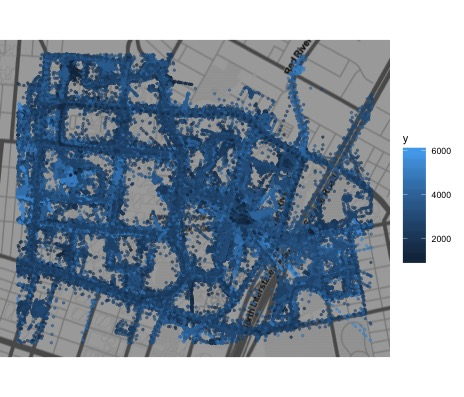
\includegraphics[width=90mm,keepaspectratio]{Images/original_data_plot.jpg}
\caption{Observed data \label{fig:1}}
\end{figure}

Second, Katzfuss and Cressie suggest de-trending to adjust for any large-scale spatial variation and any key covariates.  We plotted the raw data versus longitude, latitude, and temperature.  The data do not show any trend by latitude or longitude, ruling out deterministic trends.  There is a trend by temperature, which is not surprising as lower temperatures may affect the accuracy of the radiation measurements. \\

We chose not to de-trend the data by temperature, as this introduced strange patterns in the data when plotted by latitude and longitude. \\

\begin{figure}[!ht]
\centering
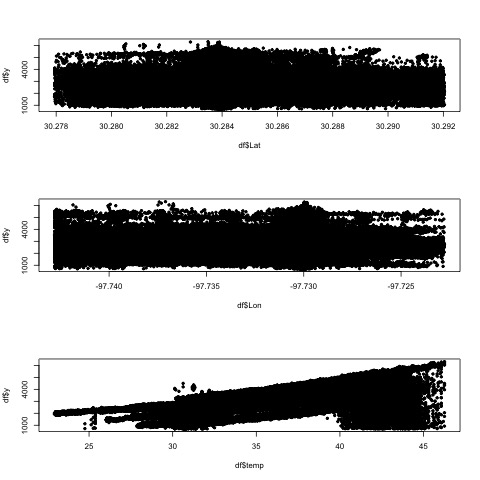
\includegraphics[width=90mm,keepaspectratio]{Images/detrending_plots.jpg}
\caption{Data by Latitude, Longitude and Temperature \label{fig:2}}
\end{figure}

\underline{Transformation to Normality}\\
Third, Katzfuss and Cressie recommend that the data be checked for approximate normality and transformed if necessary.  The radiation data is in the form of counts (intensity measurements) and is likely Poisson, so we use an Anscombe transformation to induce normality.  A histogram of the normalized observations $(y.norm)$ confirm this transformation was successful.  Note that Anscombe back-transformations can lead to a biased result, and so we use the following transform and back-transform. \\

\myindent $x \rightarrow 2\sqrt(x + \frac{3}{8})$\\
\myindent $y \rightarrow \left(\frac{y}{2}\right)^2 - \frac{1}{8}$ 
\myindent (instead of the direct algebraic inverse, where $\frac{3}{8}$ is subtracted.)

\begin{figure}[!ht]
\centering
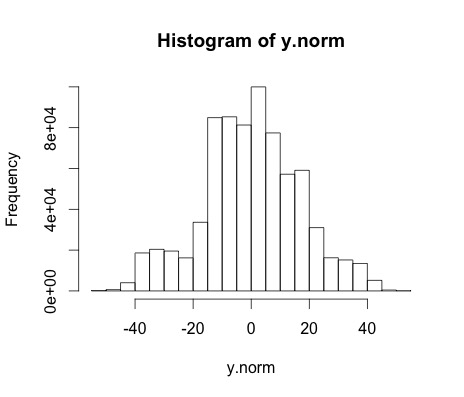
\includegraphics[width=90mm,keepaspectratio]{Images/histogram_ynorm.jpg}
\caption{Anscombe-Transformed Responses \label{fig:3}}
\end{figure}

\newpage
\subsection{Basis Function Generation}

The choice of the basis functions is a very important step in the model specification for FRK. In fact, the matrix $S$ allows us to represent the covariance structure as a linear combination of some basis function $S_1(\bm{u}), \dots, S_r(\bm{u})$, which results in a loss of information with respect to the full covariance representation.

The choice of the basis functions has to combine two goals. First of all, we should choose a number of basis functions $r \ll n$ in order to see an actual gain in terms of computational efficiency. Moreover, the basis functions have to be multiresolutional, that is, they should be allowed to capture multiple scales of variation in the covariance structure. In practice, there are a few smooth basis functions with large support (the limit case is the constant basis function, that is already implied in the centering step), and many spiky basis functions with small support. 

The choice of the basis functions involves three separate problem: the choice of the type, the number $r$ and the locations. The basis functions do not have to be necessarily orthogonal. In this work, we use bisquare functions, i.e. functions of the form
\begin{equation*}
f(r) = \begin{cases}
\left[ 1 - \left( \frac{r}{c} \right)^2 \right]^2 & r \leq c
\\
0 & r > c
\end{cases}
\end{equation*}
where $c$ represents the resolution of the function and $r$ is the euclidean distance of the coordinate from the center of the function. The number of basis functions $r$ is chosen heuristically, in such a way that it can represent well the domain but that it does not compromise the performance of the algorithm. As far as the locations are concerned, they should cover as much as possible the spatial domain of interest (the prediction grid), and they should not overlap for different basis functions.

In this work we use a total of $r = $ basis functions with three different resolutions. In particular, $r_1 = 9$ functions have a low resolution $c_1 = 5 \cdot 10^{-3}$, $r_2 = 16$ functions have an intermediate resolution $c_2 = 2 \cdot 10^{-3}$ and $r_3 = 25$ functions have a high resolution $c_3 = 10^{-3}$. 

\textbf{Check and try again to use resolution = 1.5 times the shortest distance between the center of any of the functions with that resolution [see Cressie, pag 6].}

\begin{figure}[!ht]
\centering
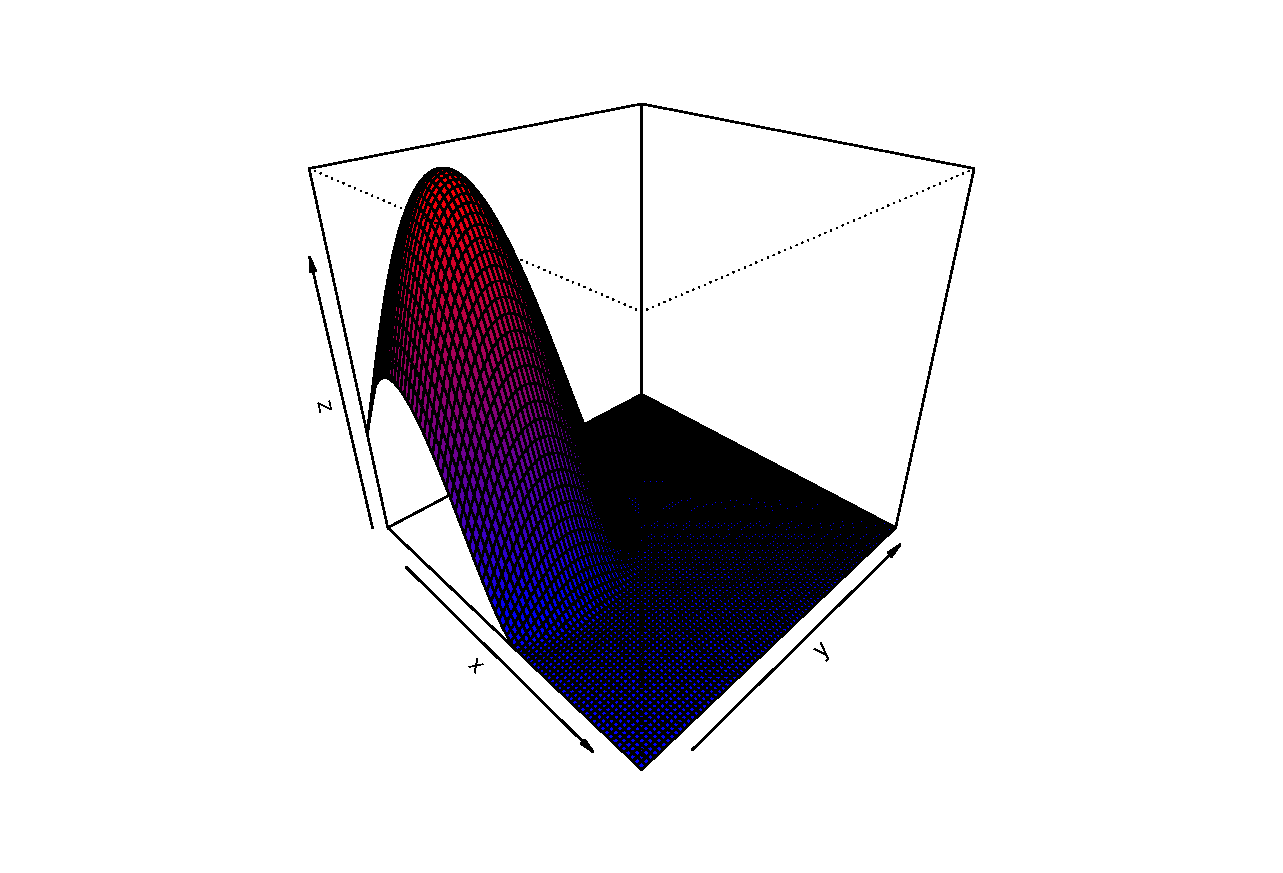
\includegraphics[width=0.55\columnwidth]{./Images/res1}
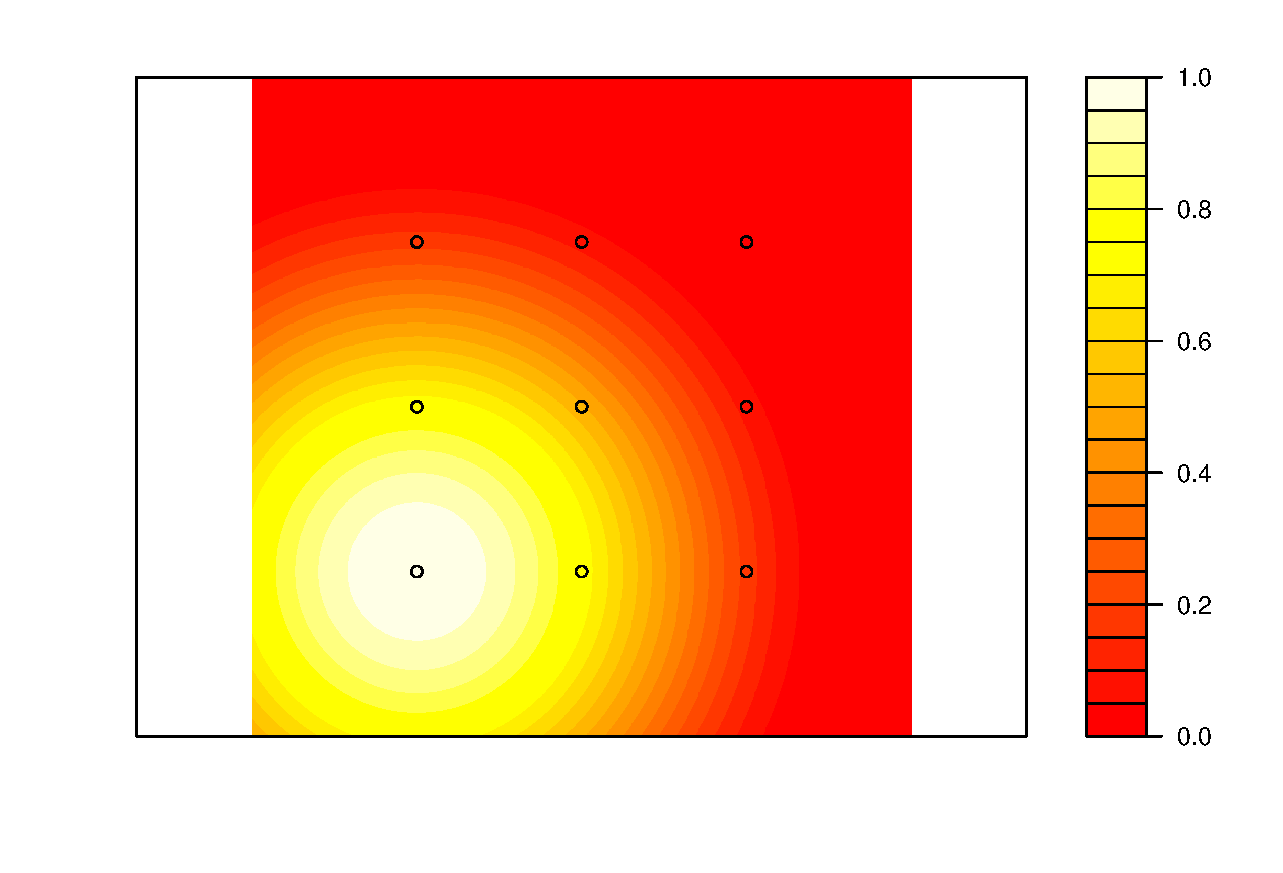
\includegraphics[width=0.44\columnwidth]{./Images/res11}
\caption{}
\label{fig:res1}
\end{figure}

\begin{figure}[!ht]
\centering
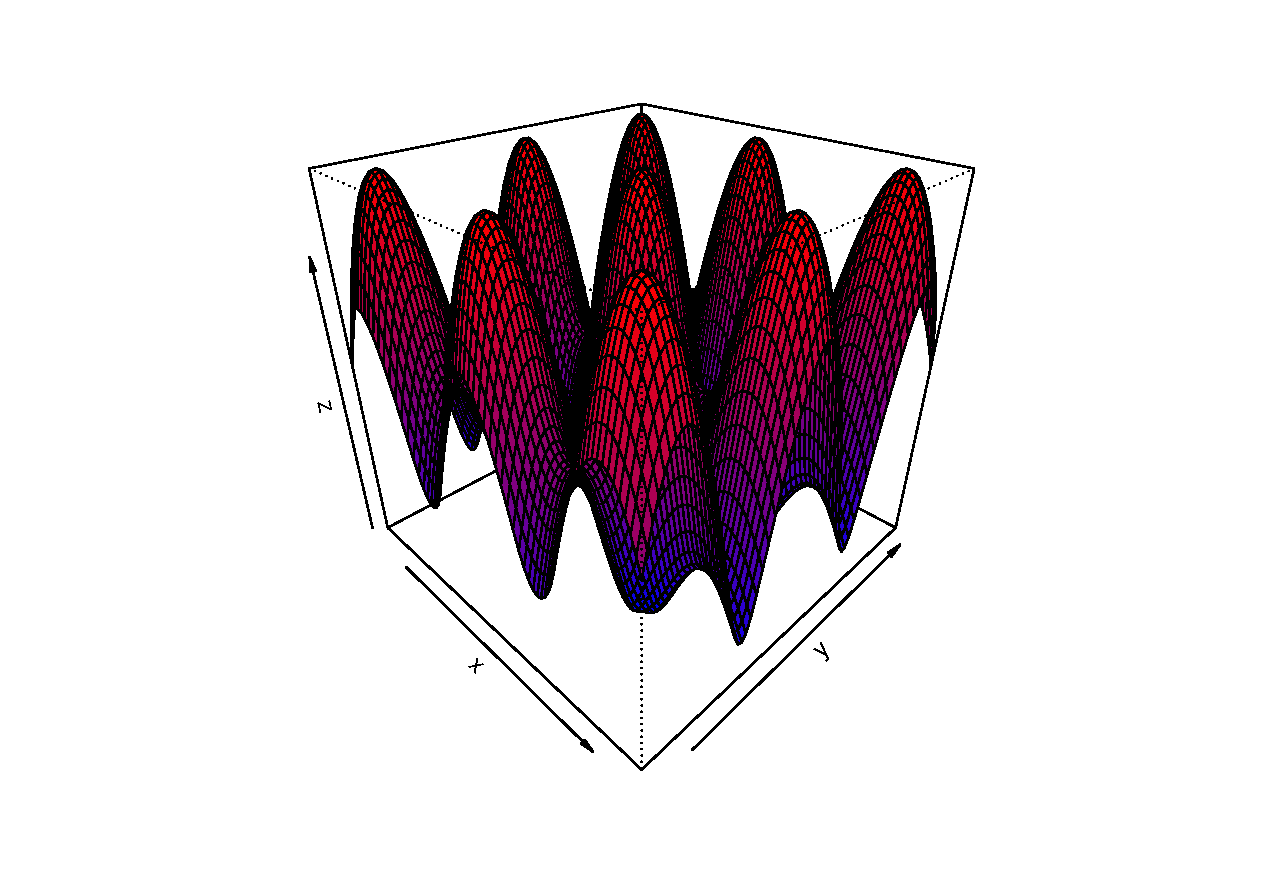
\includegraphics[width=0.55\columnwidth]{./Images/res2}
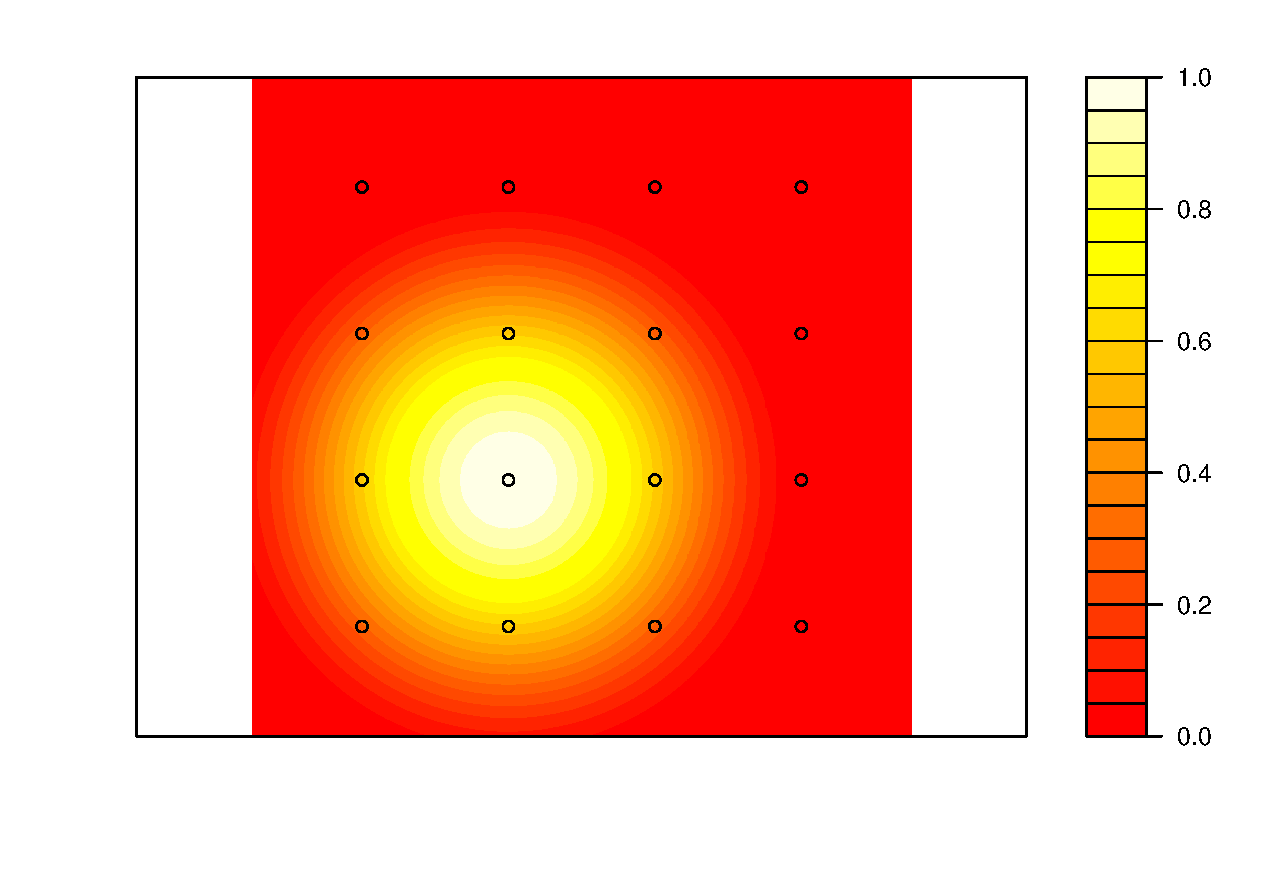
\includegraphics[width=0.44\columnwidth]{./Images/res21}
\caption{}
\label{fig:res2}
\end{figure}

\begin{figure}[!ht]
\centering
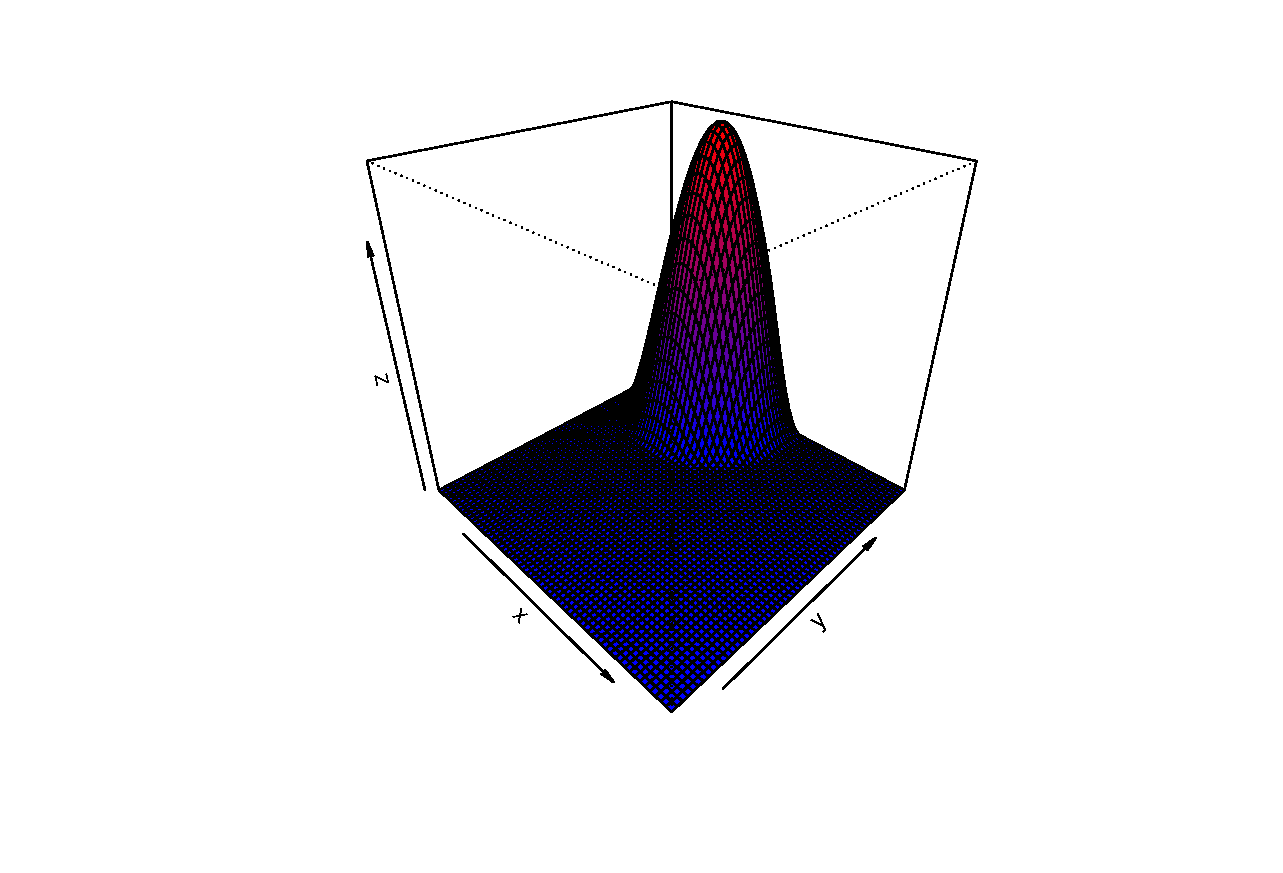
\includegraphics[width=0.55\columnwidth]{./Images/res3}
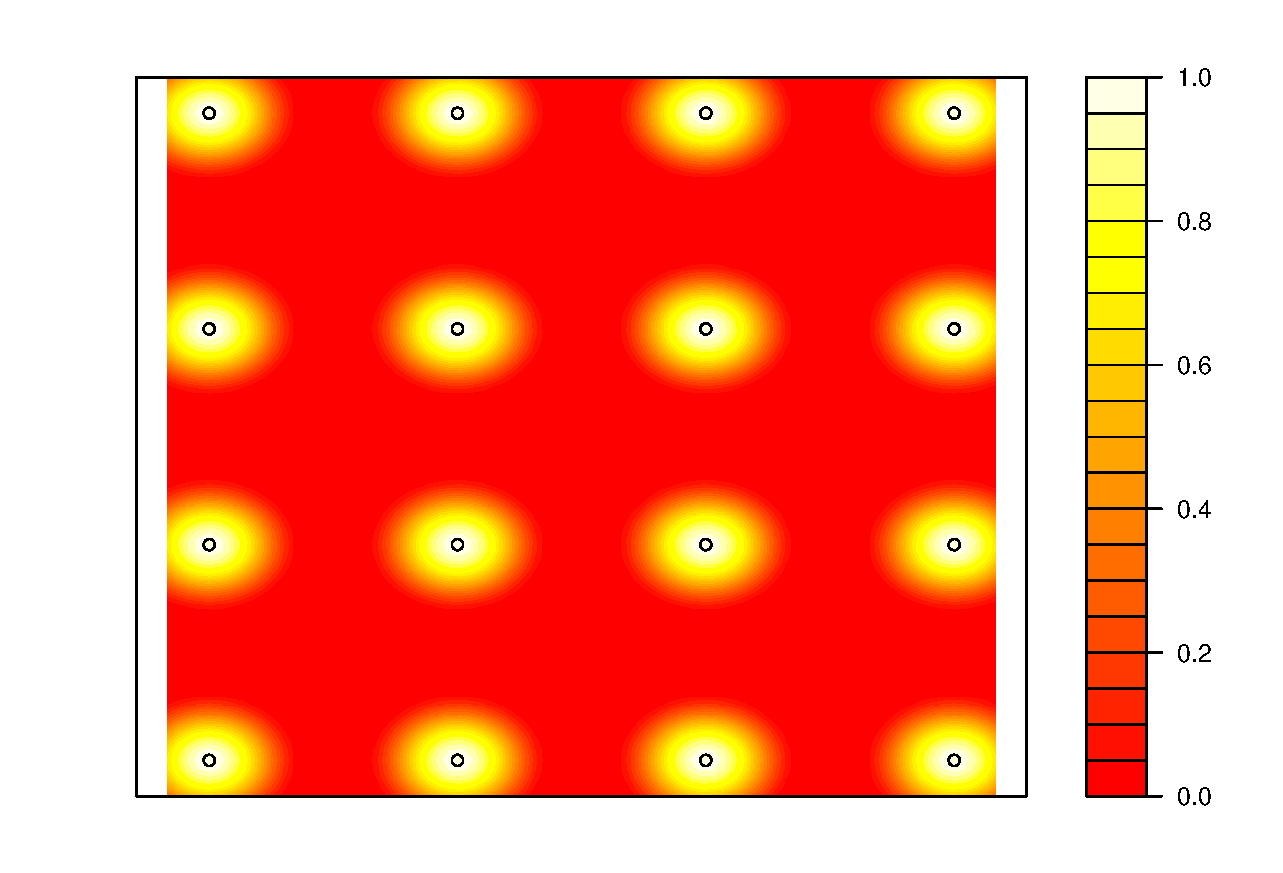
\includegraphics[width=0.44\columnwidth]{./Images/res31}
\caption{}
\label{fig:res3}
\end{figure}

\subsection{Estimation of $\sigma^2_{\epsilon}$ via Semivariogram}

The FRK model specifies that $n$ measurements are modeled as $Z(s_i) = Y(s_i) + \epsilon(s_i)$, where $s_i$ are locations in the region of interest, and $\epsilon(s_i)$ is additive measurement error.\\

As detailed above, the measurement error is assumed to be independent of $Y(s_i)$ and normally distributed as $\epsilon(s_i) \sim N(0,\sigma^2_\epsilon \nu_\epsilon (s_i))$.  The $\nu_\epsilon (s_i)$ component is a function that is assumed to be known, which describes the random spatial variation.  As with the CO2 data, we assume $\nu_\epsilon (s_i)$ is a constant function equal to 1 at every location, as we assume that random spatial variation is constant over the campus. \\

This leaves us with $\sigma^2_\epsilon$ to estimate. \\

Katzfuss and Cressie note that $\sigma^2_\epsilon$ may be specified in advance, if there is previous knowledge about measurement error for the instrument being used.  We do not assume prior knowledge of $\sigma^2_\epsilon$. \\

The semivariogram estimation method presented in Katzfuss and Cressie is known as the 'Robust Cressie Variogram.'  \\

\myindent $\bullet$ $2\gamma(h) = \left( \frac{1}{|N(h)|} \sum_{N(h)}|
\frac{\tilde{Z}(s_i)}{\sqrt{\nu_\epsilon (s_i)}} - 
\frac{\tilde{Z}(s_j)}{\sqrt{\nu_\epsilon (s_j)}} - 
|^{.5} \right)^4 / \left(0.457 + 0.494 / |N(h)|\right)$ \\

\myindent\myindent where: \\
\myindent \myindent  $\tilde{Z}(s_i)$ are the normalized, de-trended data. \\
\myindent \myindent $N(h) = {(i,j): ||s_i - s_j|| \in [h - \delta, h + \delta ] }$, \\
\myindent \myindent \myindent the set of all indices for location pairs roughly $h$ distance apart.\\

\myindent $\bullet$ Then straight line $\hat{\gamma}(h) = \hat{\gamma}(0) + bh$ is fit, and $\sigma^2_\epsilon = \hat{\gamma}(0)$.\\

(For further detail on this methodology, see Cressie and Hawkins (1980), Cressie (1985), and Kang et al. (2010). \\

We use this method to estimate a semi-variogram for the data, and then fit a straight line to the semivariogram and let $\hat{\sigma}^2_\epsilon$ be equal to the intercept.  Our resulting estimate is $\hat{\sigma}^2_\epsilon$ = 106.3635. \\

We did remove the police station measurements in the calculation of this semivariogram.  The police car carrying the measurement device parked in the police station lot overnight, so there were a disproportionate number of measurements at this location, including specifically nighttime measurements where cooler temperatures mean the measurement device is more prone to error. \\

This was considerably higher than the estimate obtained for the Katzfuss and Cressie simulated CO2 data.  However, their data was simulated with $\sigma2_\epsilon = 0.25$, and our normalized data has a range of -51 to 54, with a total variance of 287, so our result is reasonable. To check reasonableness, we split the region of interest into four quadrants and calculated semivariograms for each quandrant to ensure that they yielded comparable $\hat{\sigma}^2_\epsilon$ estimates. Estimates were similar in all regions, and did not differ significantly from the overall estimate.   The data is known to have some outliers which affect the variance.\\


\subsection{Estimation of $\sigma^2_{\xi}$ and $K$ via EM Algorithm}

The next step of the Fixed Rank Kriging process is to estimate the parameters $\sigma^2_{\xi}$ and $K$.  \\

As described above, $K$ is the $(r x r)$ covariance matrix, where $r$ is the number of basis functions selected.  $K$ represents the covariance in the spatial-random-effects (SRE) model.\\

$\sigma^2_{\xi}$ is the fine-scale variance in the SRE model, accounting for error introduced to the model through the dimension reduction. \\

Katzfuss and Cressie suggest two methods for estimating these parameters: Method of Moments and the EM Algorithm.  We have implemented the EM algorithm to estimate these values.  (Details for the formulas are included previously in the Methods section; R code is included in the appendix.)\\

We obtain an estimated $\hat{\sigma}^2_{\xi} = 174.4245$.  The R code saves $\hat{\sigma}^2_{\xi}$ and $\hat{K}$ as part of the EM function output.\\

\subsection{Fixed Rank Kriging: Smoothing and Prediction}

Stuff.\\


%%%%%%%%%%%%%%%%%%%%%%%%%%%%%%%%%%%%%%%%%%%%%%%%%%%%%%%%%%%%%%%%%%%%
%%                     RESULTS                                    %%
%%%%%%%%%%%%%%%%%%%%%%%%%%%%%%%%%%%%%%%%%%%%%%%%%%%%%%%%%%%%%%%%%%%%
\newpage
\section{3. Results}

Using a uniform set of basis functions, predicted kriging values are shown in the heatmap below, followed by a plot of the kriging variance. \\

\begin{figure}[h!]
\centering
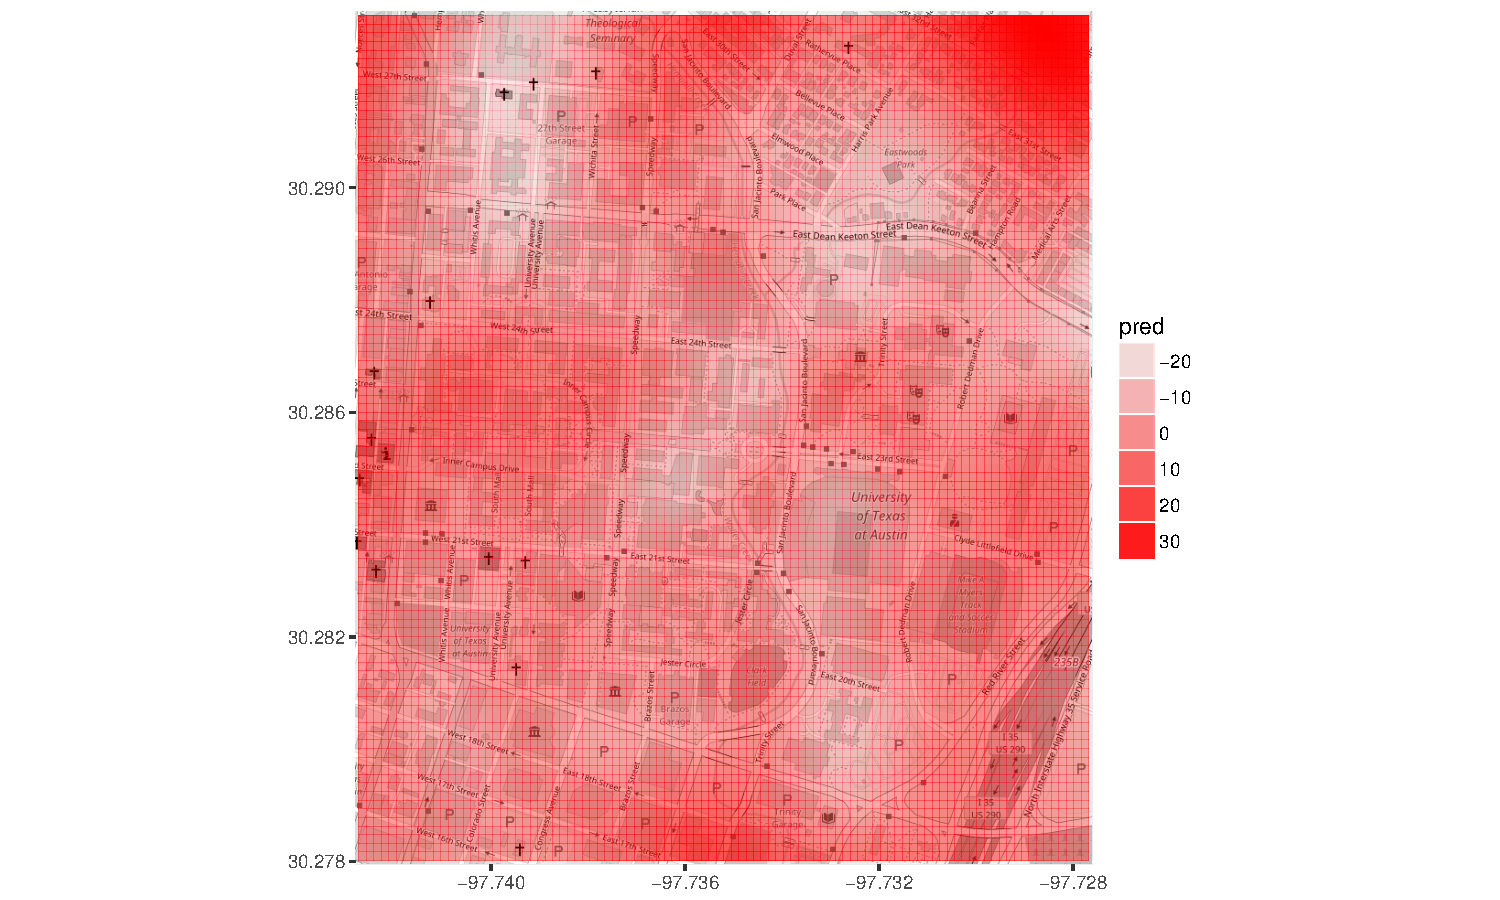
\includegraphics[width=160mm,keepaspectratio]{Images/pred.pdf}
\caption{Predicted values, uniform basis \label{fig:4}}
\end{figure}

\begin{figure}[h!]
\centering
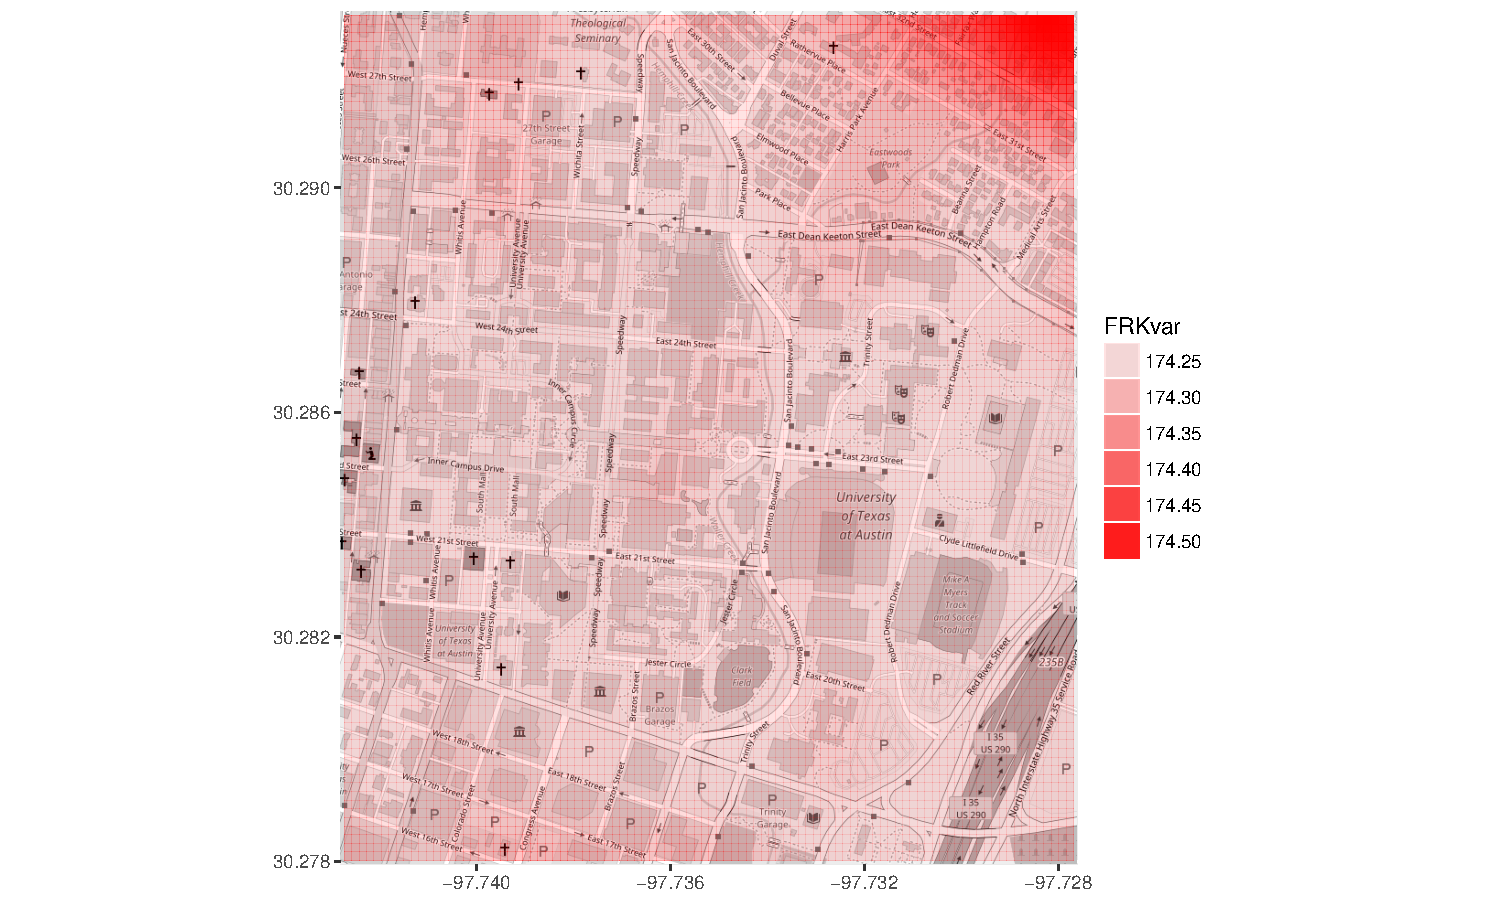
\includegraphics[width=160mm,keepaspectratio]{Images/var.pdf}
\caption{FRK variance, uniform basis \label{fig:5}}
\end{figure}

\begin{figure}[h!]
\centering
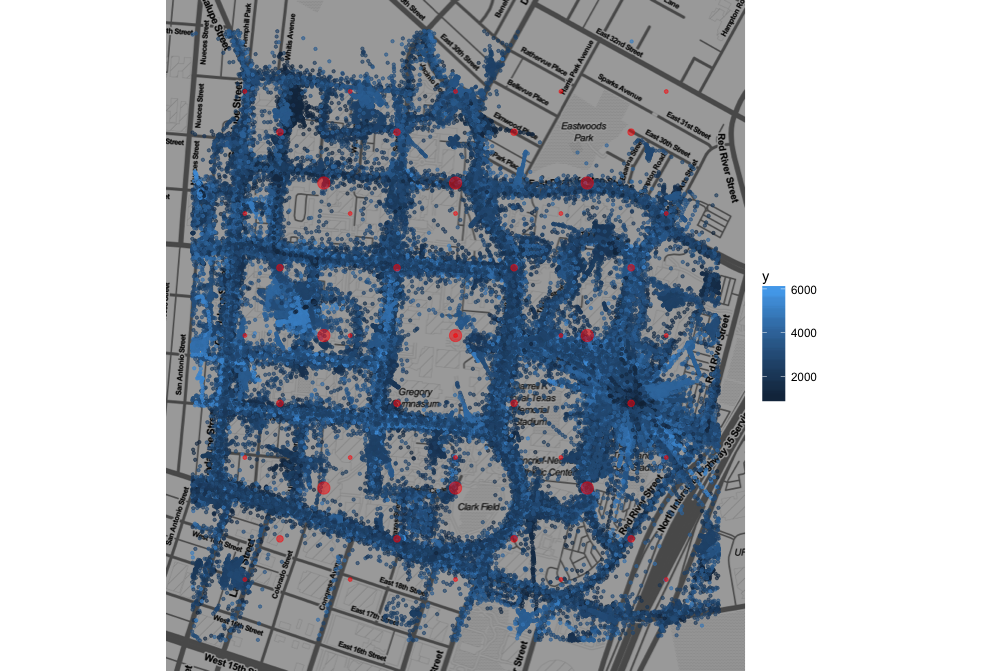
\includegraphics[width=160mm,keepaspectratio]{Images/data_grid.png}
\caption{Observed data and basis function centers \label{fig:6}}
\end{figure}

We noticed an area in the top right of very high variance.  This issue is caused by very sparse observed data coverage in the top right area of the grid; there is one blue point by itself which is near East 32nd Street.  There are no other close points informing the kriging estimate in this area of the grid, and compounding the issue, there are two spiky basis centers quite close to this point. \\

To address this issue, we adjusted the basis centers by removing the two spiky centers in this corner.  We justified this by noting that kriging is not intended to extrapolate into new regions without surrounding estimates to inform the prediction.  Of course a lone point is going to have a high kriging variance, when none of its neighbors are near. The result of this adjustment is below. \\

\begin{figure}[h!]
\centering
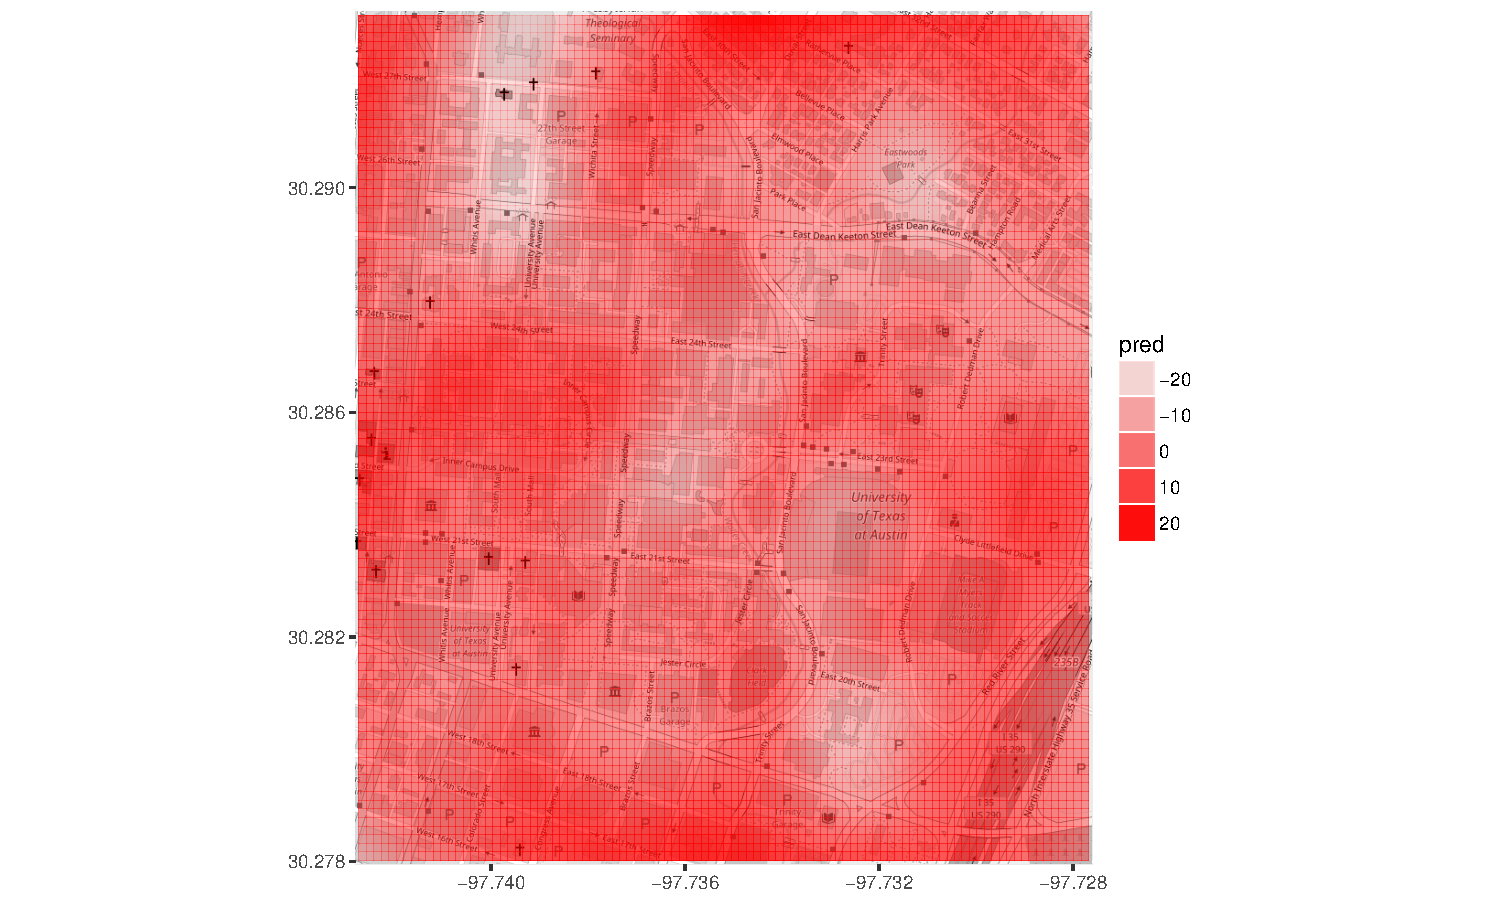
\includegraphics[width=160mm,keepaspectratio]{Images/pred_newgrid.pdf}
\caption{Predicted values, adjusted basis \label{fig:7}}
\end{figure}

\begin{figure}[h!]
\centering
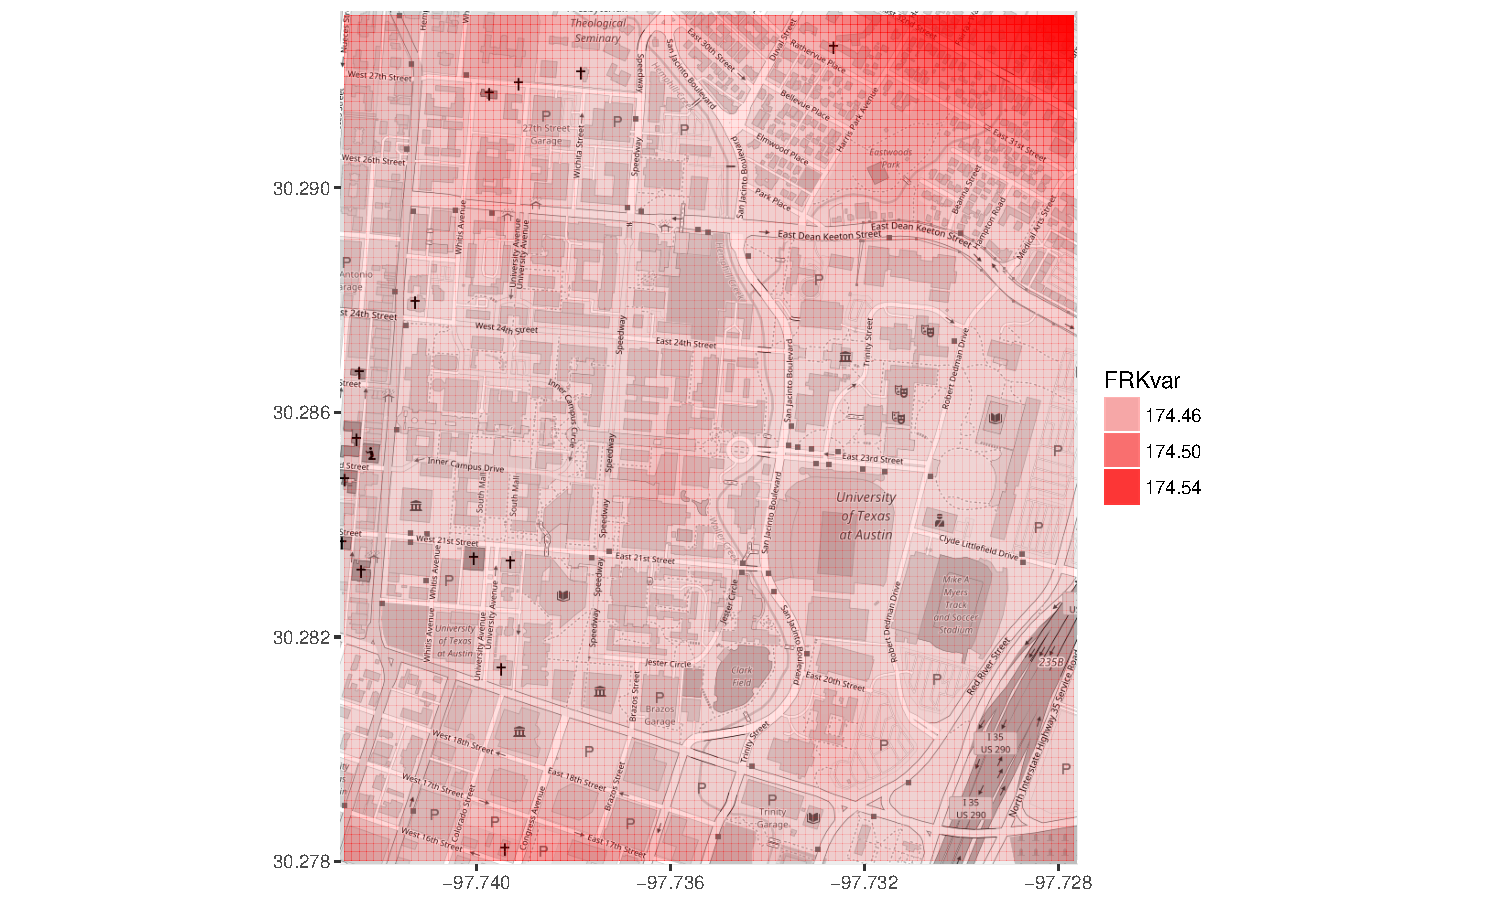
\includegraphics[width=160mm,keepaspectratio]{Images/var_newgrid.pdf}
\caption{FRK variance, adjusted basis \label{fig:8}}
\end{figure}

\begin{figure}[h!]
\centering
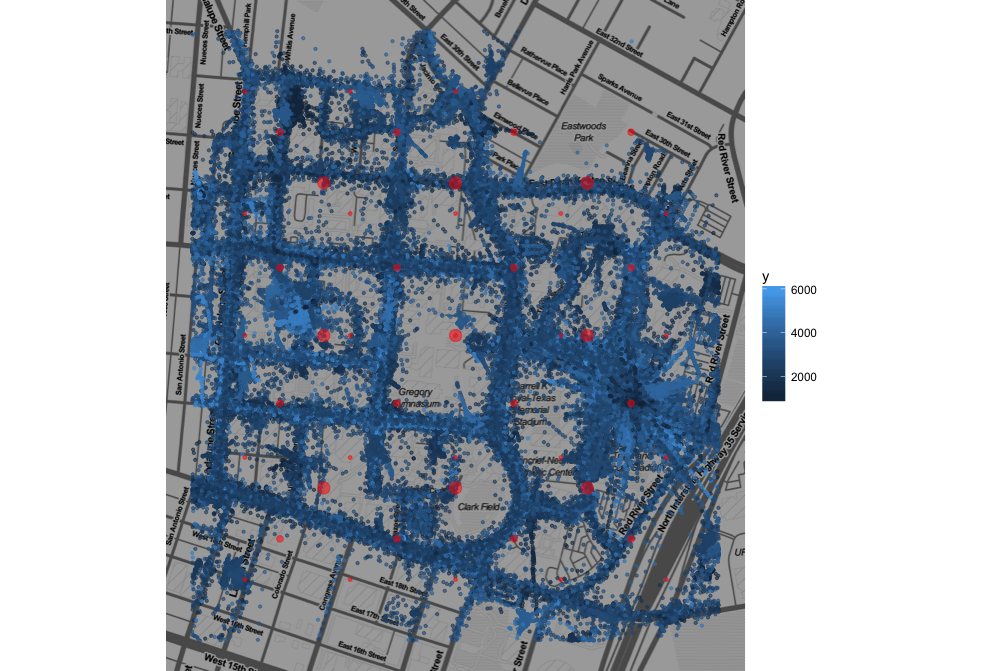
\includegraphics[width=160mm,keepaspectratio]{Images/data_grid_new.png}
\caption{Observed data and adjusted basis function centers \label{fig:9}}
\end{figure}

The result of this adjustment yields desirable results for the predicted data.  The kriging variance is nearly uniform across the predicted grid of locations, with the area of high variance in the top right region reduced in size.\\

Finally, we include a histogram of the observed versus predicted residual for the kriging function applied to the observed locations.  These values should be normally distributed to indicate goodness of model fit.\\

\begin{figure}[h!]
\centering
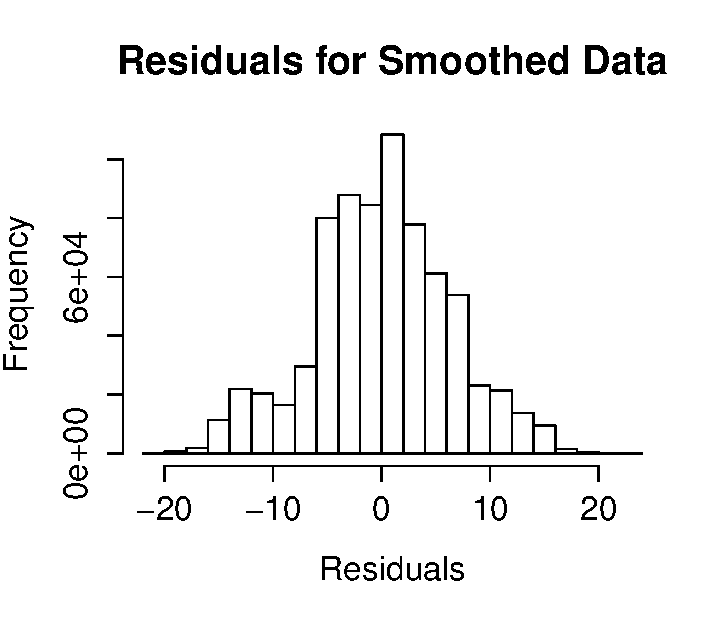
\includegraphics[width=90mm,keepaspectratio]{Images/Residuals_for_smoothing.pdf}
\caption{Residuals \label{fig:10}}
\end{figure}



%%%%%%%%%%%%%%%%%%%%%%%%%%%%%%%%%%%%%%%%%%%%%%%%%%%%%%%%%%%%%%%%%%%%
%%                     DISCUSSION                                 %%
%%%%%%%%%%%%%%%%%%%%%%%%%%%%%%%%%%%%%%%%%%%%%%%%%%%%%%%%%%%%%%%%%%%%
\newpage
\section{4. Discussion}

Discussion goes here. \\

DO NOT FORGET TO CHECK NORMALITY OF RESIDUALS!!!!!!!\\

%%%%%%%%%%%%%%%%%%%%%%%%%%%%%%%%%%%%%%%%%%%%%%%%%%%%%%%%%%%%%%%%%%%%
%%                     R APPENDIX & DOCUMENTATION                 %%
%%%%%%%%%%%%%%%%%%%%%%%%%%%%%%%%%%%%%%%%%%%%%%%%%%%%%%%%%%%%%%%%%%%%
\newpage
\section{5. R Code Appendix}

\subsection{Documentation Source}
All project documentation and source code is available in the following github repository. \\

\myindent \underline{https://github.com/jstarling1/spatialsmoothing}

\subsection{R Code: Main Launcher File}


\subsection{R Code: Main Launcher File}


% 
% \subsection{R Code: Main Analysis Code}
% \linespread{1} % Line spacing for R code section.
% \lstinputlisting[language=R,breaklines=true]{"/Users/jennstarling/UTAustin/2016_Fall_SDS 383C_Statistical Modeling 1/Final Project/penalized-matrix-decomp/R Code/383C_FinalProject_RCode.R"}
% 
% \subsection{R Code: Penalized Matrix Decomposition Functions}
% 
% %% Display R script.
% \lstinputlisting[language=R,breaklines=true]{"/Users/jennstarling/UTAustin/2016_Fall_SDS 383C_Statistical Modeling 1/Final Project/penalized-matrix-decomp/R Code/Penalized_Matrix_Decomp_Functions.R"}

\end{document}